\documentclass[a4paper,10pt]{report}
\usepackage[utf8]{inputenc}
\usepackage{graphicx}
\usepackage[francais]{babel}

% Title Page
\title{TP Arbres recouvrants}
\author{Arnaud Cojez \and Matthieu Caron}


\begin{document}

\maketitle

\chapter{Implémentation}

\section{Structure de Donnée utilisée}
Pour notre représentation de graphe on a trois classes différente,
\begin{itemize}
 \item la classe Sommet qui contient la liste des Aretes qui lui sont associés et une couleur.
 \item la classe Arete qui contient deux sommets
 \item la classe Graph qui contient la liste de toutes les aretes ainsi que la liste de tous les sommets.
\end{itemize}

\section{Ce qui a été fait}
Nous avons implémenté les graphes, les algorithmes de construction de MST, des tests de performance avec une moyenne faite sur 50 exécutions de chaque algo sur des graphes différents, ainsi que l'export et l'import de graphe sous format texte. 

\section{Les Algorithmes de construction de MST}
Les algoritmes implémentés sont les suivants : Algorithme de Prim et algorithme de Kruskal.

\chapter{Tests}

\begin{center}
  \begin{figure}[ht]
    \label{color}
    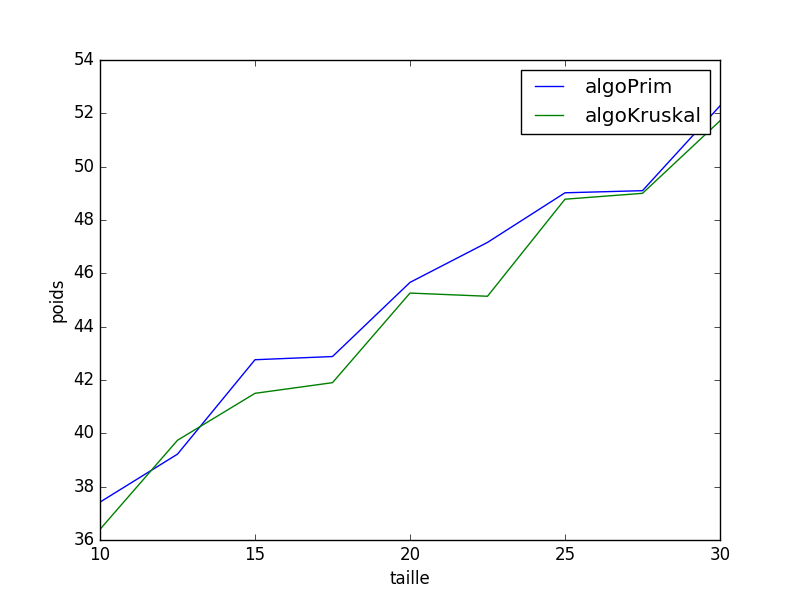
\includegraphics[scale=0.5]{poids(taille).png}
    \caption{Poids de l'arbre en fonction du nombre de sommets}
  \end{figure} 
\end{center}

\begin{center}
  \begin{figure}[ht]
    \label{color}
    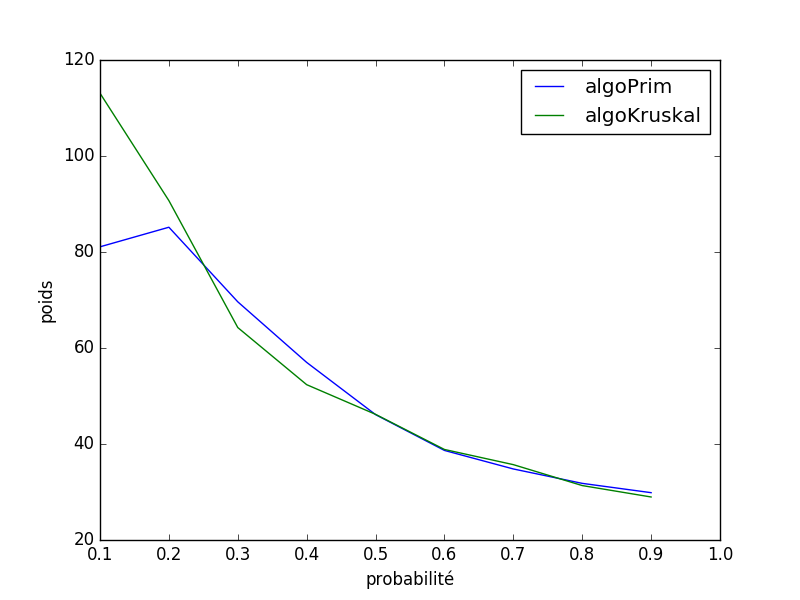
\includegraphics[scale=0.5]{poids(probabilite).png}
    \caption{Poids de l'arbre en fonction du nombre de branches}
  \end{figure} 
\end{center}

\begin{center}
  \begin{figure}[ht]
    \label{color}
    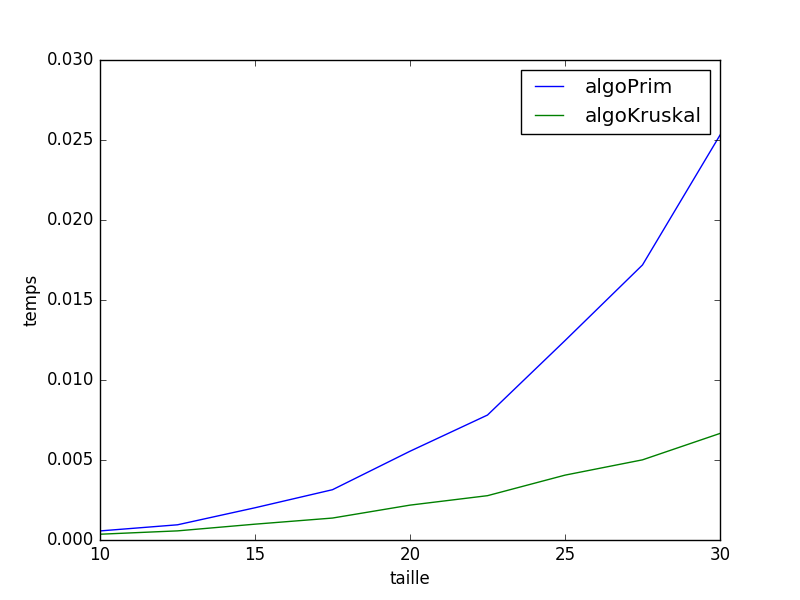
\includegraphics[scale=0.5]{temps(taille).png}
    \caption{Temps d'éxecution des algorithmes en fonction du nombre de sommets}
  \end{figure} 
\end{center}

\begin{center}
  \begin{figure}[ht]
    \label{color}
    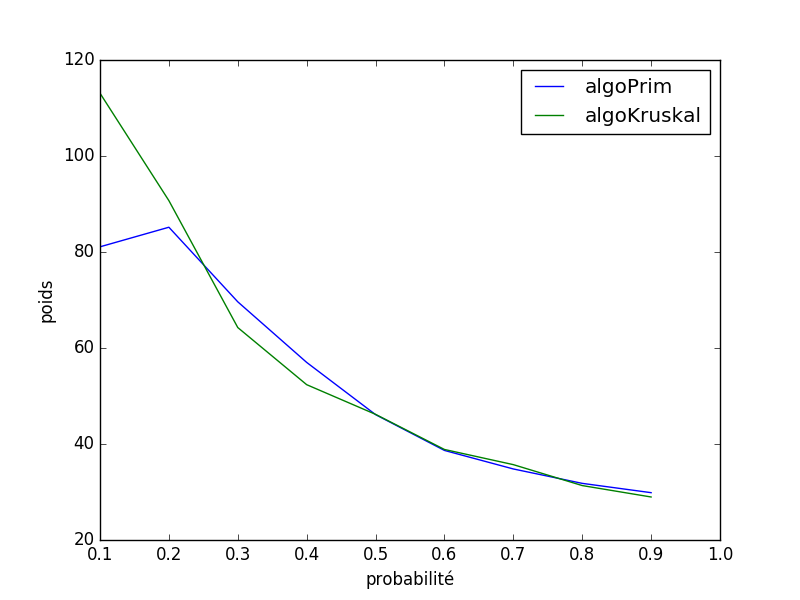
\includegraphics[scale=0.5]{poids(probabilite).png}
    \caption{Temps d'éxecution des algorithmes en fonction du nombre de branches}
  \end{figure} 
\end{center}

\chapter{Observations}


\section{Efficacité sur le poids}

On constate que même si l'algorithme Kruskal est plus efficace que le Prim avec un faible nombre d'arêtes, les 2 algorithmes sont dans le même ordre d'efficacité. Que ce soit par rapport au nombre de sommets ou au nombre d'arêtes, les résultats sont proches.

\section{Efficacité en temps}

On constate que l'algorithme Kruskal est beaucoup plus rapide que l'algorithme Prim à la fois en fonction du nombre de sommets et du nombre d'arêtes.

\end{document} 